\begin{figure}
\centering
\fbox{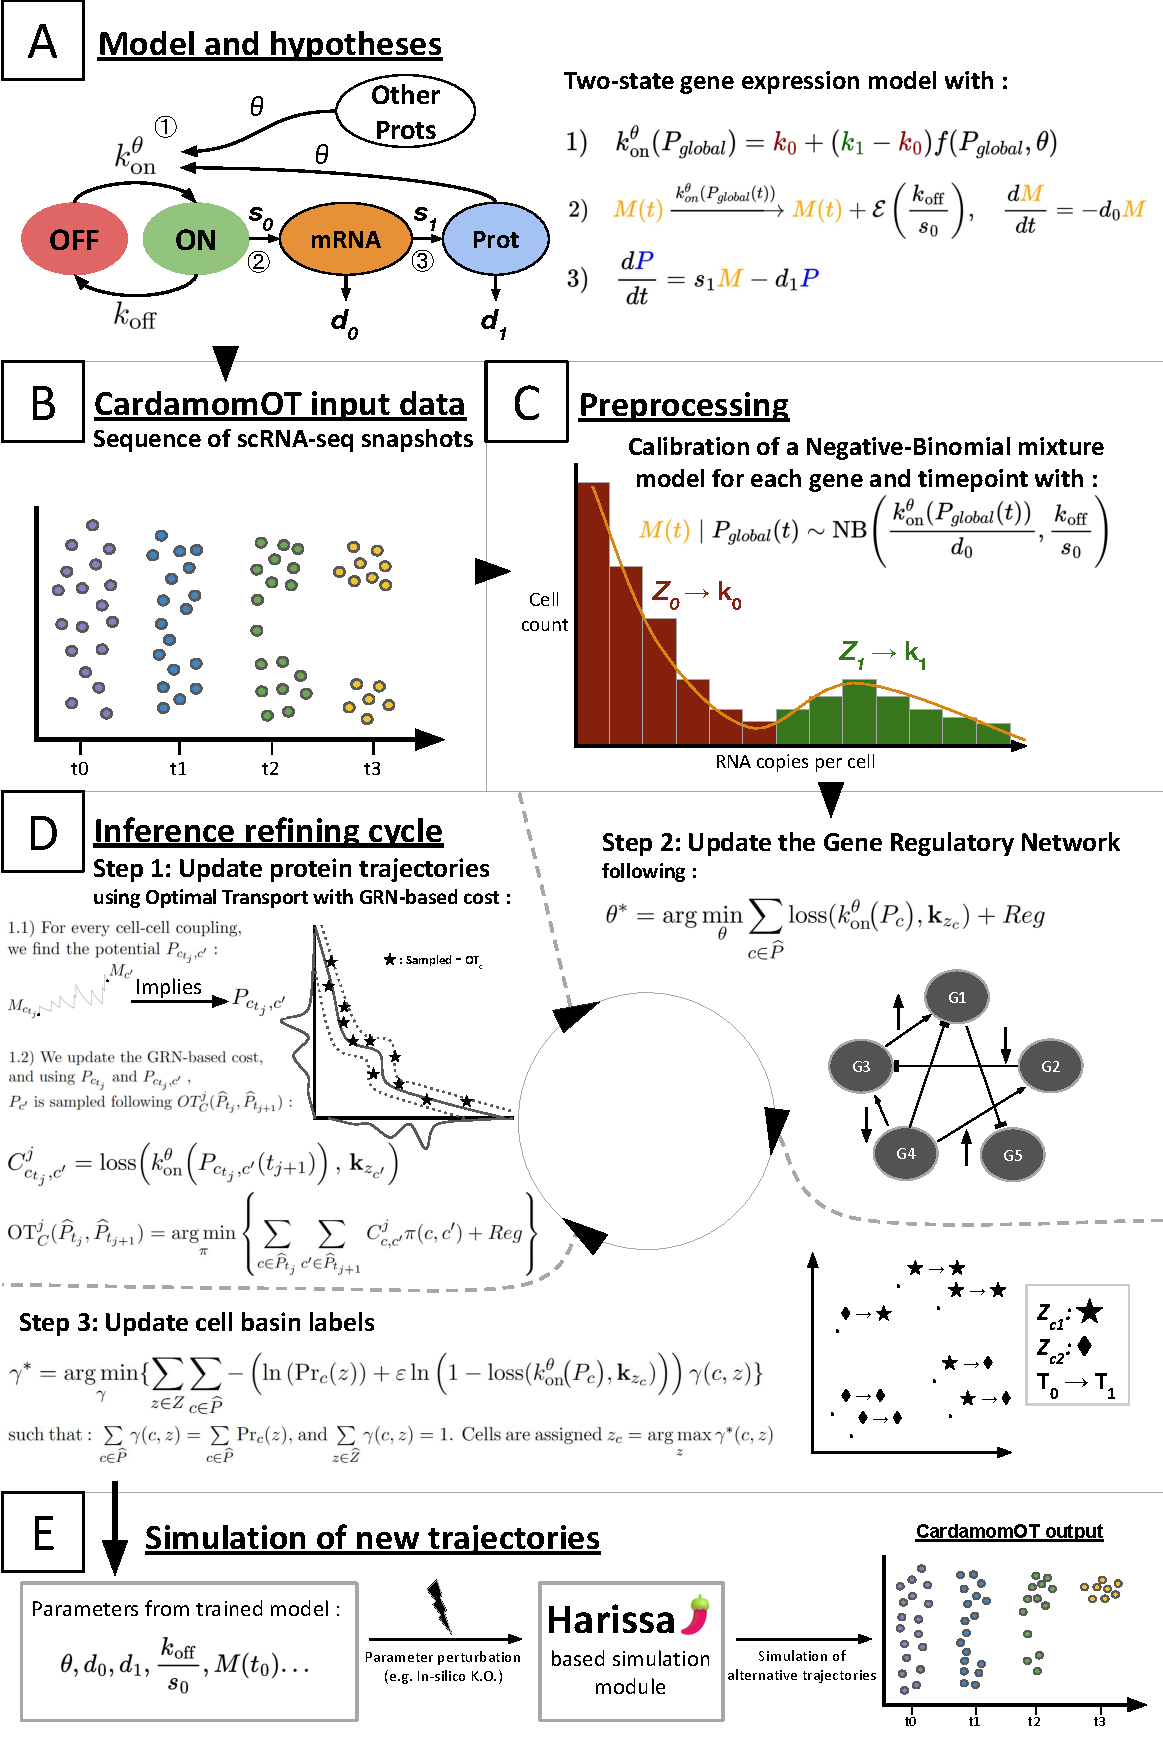
\includegraphics[width=.8\textwidth]{figure_1.pdf}}
    \caption{
CardamomOT infers gene regulatory networks (GRNs) and protein trajectories from temporal snapshots of scRNA-seq data using a mechanistic optimal transport framework. (A) The two-state gene expression model underlying the method, in which promoter switching rates are modulated by a GRN matrix $\theta$. (B) Input data consisting of independent scRNA-seq snapshots at successive timepoints. (C) Preprocessing step: a Negative Binomial mixture model is calibrated for each gene and timepoint, clustering cells into discrete promoter-activity basins. (D) Iterative EM-like inference cycle alternating between protein trajectory reconstruction via GRN-driven optimal transport (Step 1), GRN update by regression on reconstructed protein values (Step 2), and basin label refinement (Step 3). (E) The calibrated model is used as a generative module for simulating alternative trajectories and in silico perturbation experiments.}
    \label{figure1}
\end{figure}

\begin{figure}
\centering
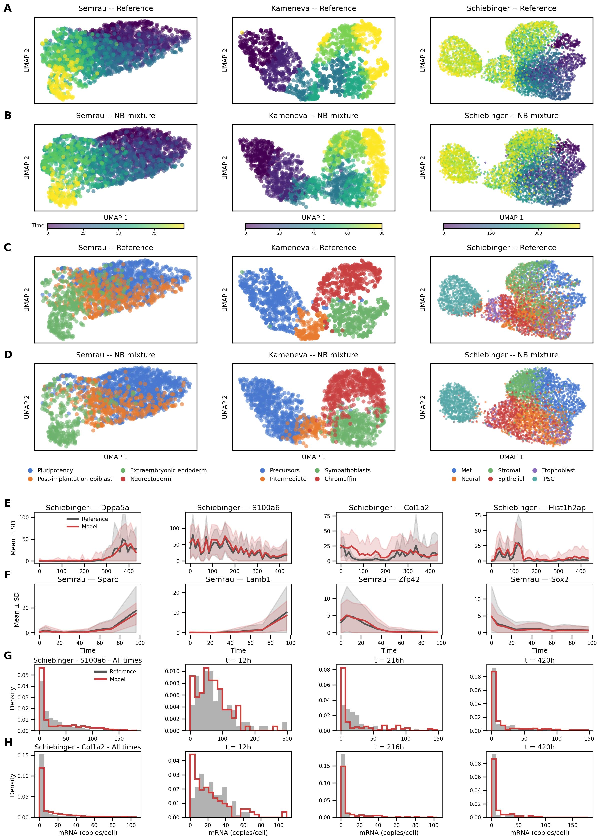
\includegraphics[width=.92\textwidth]{figure_2.pdf}
    \caption{
(A–D) UMAP embeddings of reference scRNA-seq data (A, C) and data simulated from the 
CardamomOT NB mixture model (B, D), colored by timepoint (A–B) and cell type (C–D), for 
the Semrau, Kameneva and Schiebinger datasets. (E–F) Temporal profiles of mean $\pm$ SD 
gene expression across all cells for selected key regulators, comparing reference data (gray) and model 
simulations (red), for the Schiebinger (E) and Semrau (F) datasets. (G–H) Marginal mRNA 
distributions at selected timepoints for S100a6 (G) and Col1a2 (H) in the Schiebinger dataset, showing close agreement 
between model and reference data across all timepoints.}
    \label{figure2}
\end{figure}

\begin{figure}
\centering
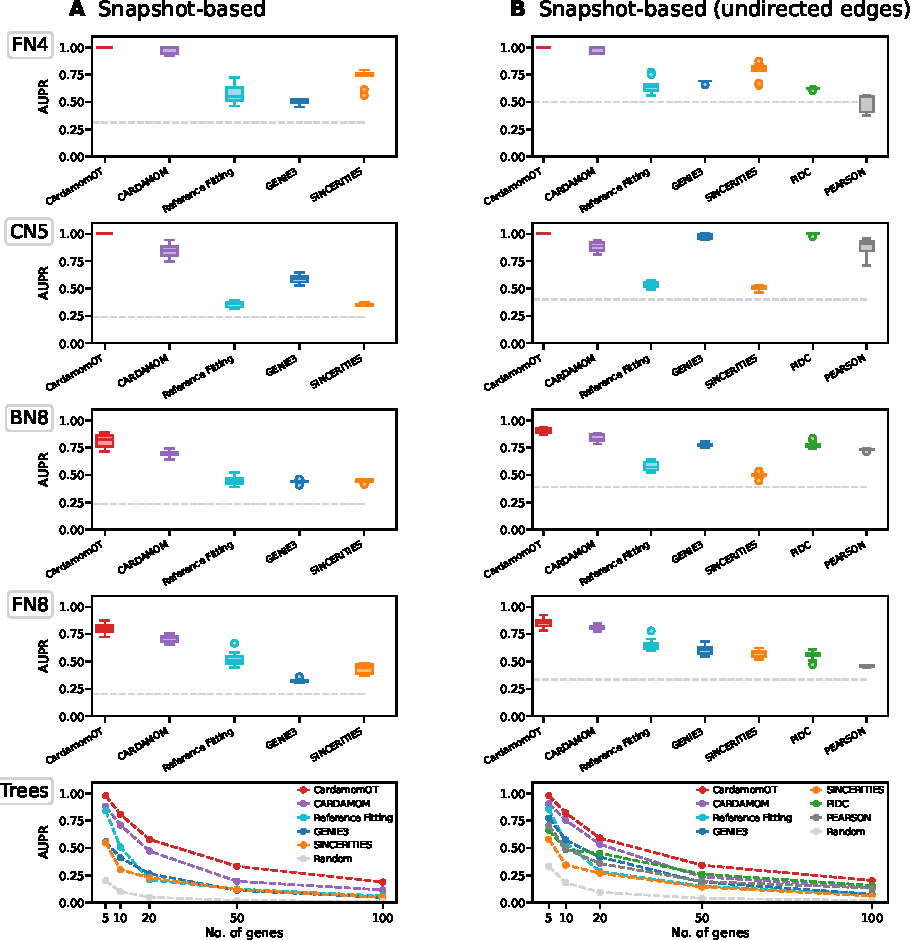
\includegraphics[width=\linewidth]{figure_3.pdf}
    \caption{CardamomOT outperforms competing methods on GRN inference benchmarks. Performance is measured by the Area Under the Precision-Recall curve (AUPR), averaged over 10 independent simulations per network. The dashed gray line indicates the random baseline. (A) Directed GRN inference from temporal snapshots on four benchmark network topologies (FN4, CN5, BN8, FN8) and tree networks of increasing size (5–100 genes). (B) Same comparison for undirected edge inference, including additional correlation-based methods (PIDC, Pearson). \firstreview{Boxplots throughout the figure show median, interquartile range (box) and 1.5x interquartile range (bars).}}
    \label{figure3}
\end{figure}

\begin{figure}
\centering
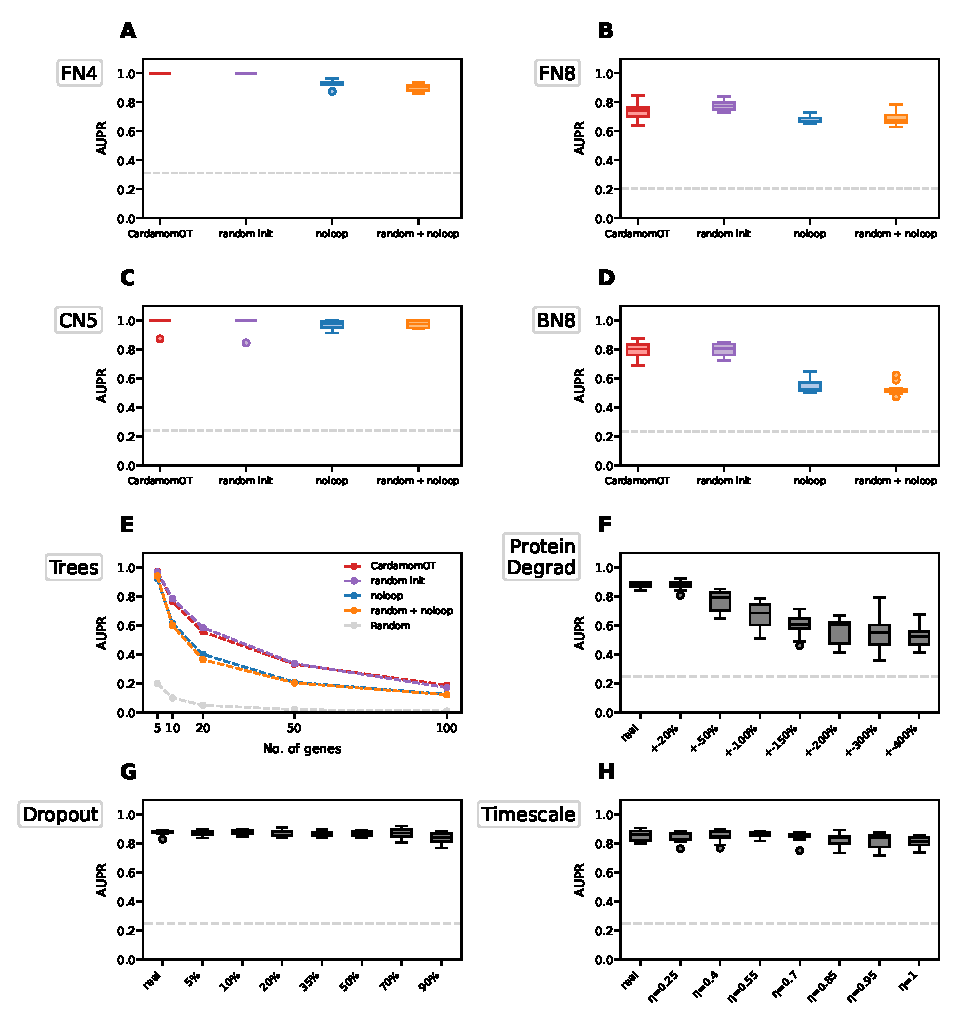
\includegraphics[width=0.95\linewidth]{figure_4.pdf}
    \caption{(A–E) Directed GRN inference performance (AUPR) \firstreview{averaged over 10 independent simulations per network} comparing CardamomOT against three ablated variants: random OT initialization (random init), removal of the loop procedure (noloop), and their combination (random + noloop), on four benchmark networks and tree topologies of increasing size. (F) Robustness to uncertainty in protein degradation rates $d_1$: AUPR averaged across 10 independent simulations for all four benchmark networks when input degradation rates are perturbed from ±20\% to ±400\% of their true values, compared to the performance obtained with the real rates. \firstreview{(G) Robustness to dropout in input data: AUPR averaged across 10 independent simulations for all four benchmark networks for base data and 7 increasing levels of binomial dropout rangin from $0\%$ (no dropout, renamed real in the figure) to $90\%$. (H) Robustness in variability in timescales: AUPR averaged across 10 independent simulations for all four benchmark networks for base data and 7 increasing levels of variability in timepoint sampling. For each replicate, inter-timepoint gaps were drawn from $\text{Dirichlet}(\alpha = 1/\eta^2)$ with endpoints fixed, where $\eta$ ranges from $0$ (equispaced timepoints, renamed real in the figure) to $1$ (uniformly sampled timepoints). Boxplots throughout the figure show median, interquartile range (box) and 1.5x interquartile range (bars).}}
    \label{figure4}
\end{figure}

\begin{figure}
\centering
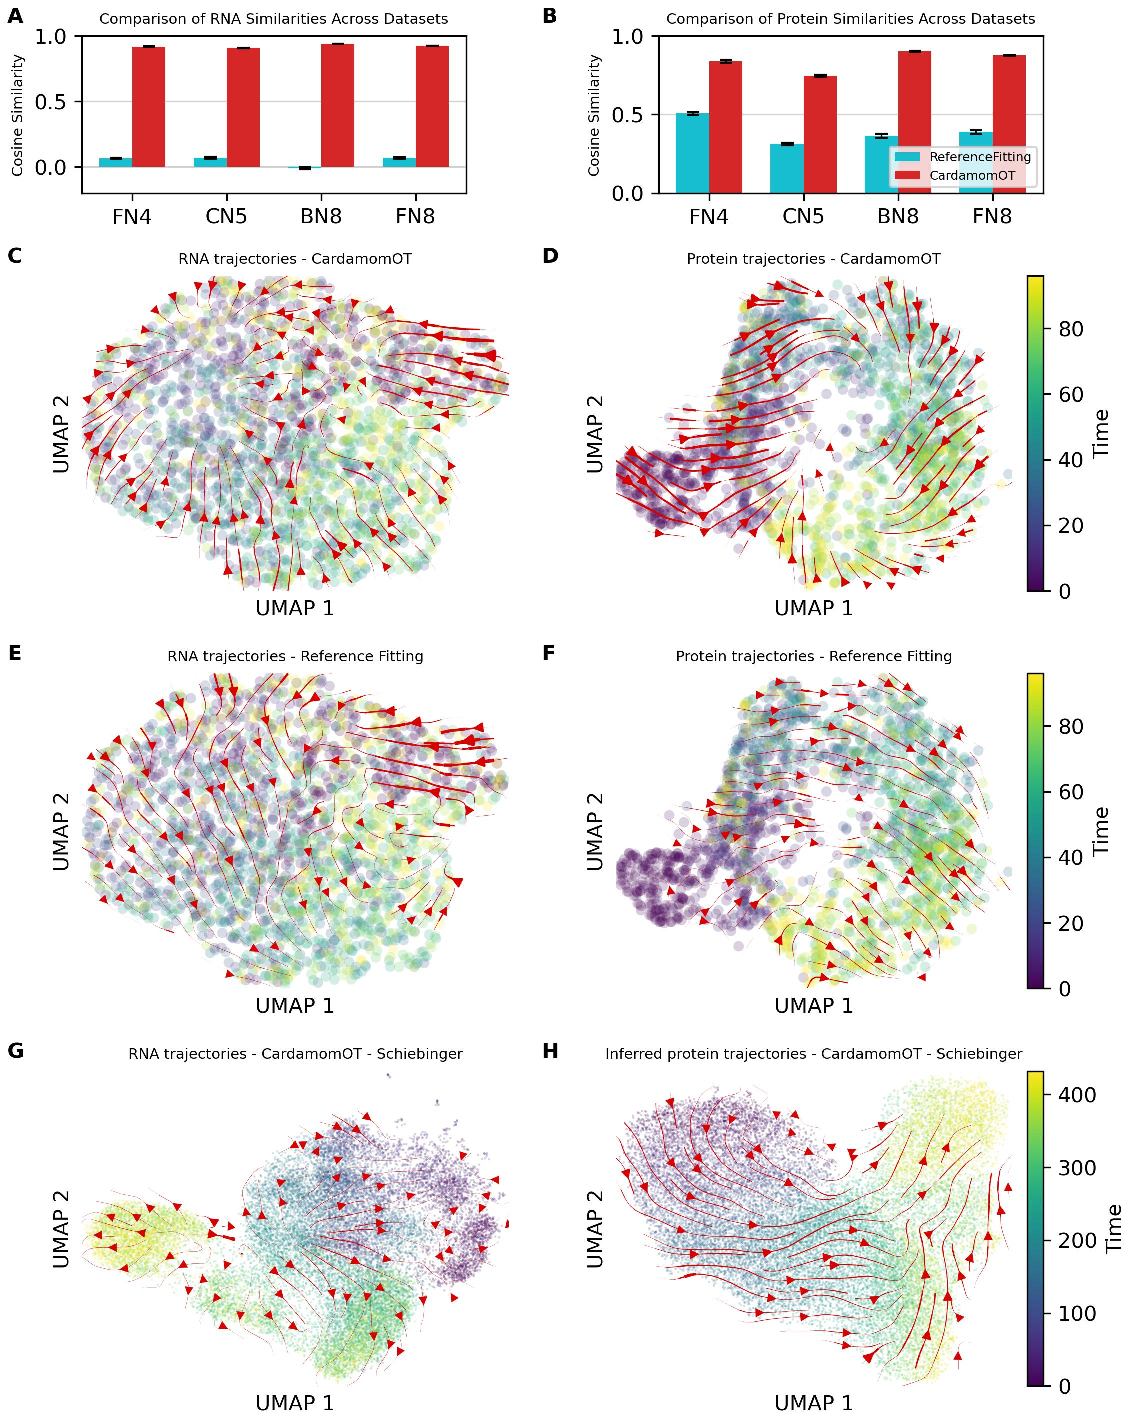
\includegraphics[width=0.98\textwidth]{figure_5.pdf}
    \caption{Evaluation of the mRNA and protein velocity fields reconstruction on 
    cross-sectional data for CardamomOT and Reference Fitting. (A--B) Weighted cosine similarity between the velocity fields 
    predicted by CardamomOT and Reference Fitting and the mechanistic ground-truth velocity 
    field, for mRNA (A) and protein (B), on four benchmark networks (BN8, FN8, CN5, FN4). 
    Bars show the mean over 5 independent simulations; error bars indicate the standard error 
    of the mean. (C--F) UMAP embeddings of RNA (C,E) 
    and protein (D,F) expression of CN5 benchmark cells, overlaid with velocity stream plots 
    from CardamomOT (C--D) and Reference Fitting (E--F). (G--H) UMAP of RNA (G) and inferred 
    protein (H) data from the Schiebinger dataset, with 
    CardamomOT velocity stream plots.}
    \label{figure5}
\end{figure}



\begin{figure}
\centering
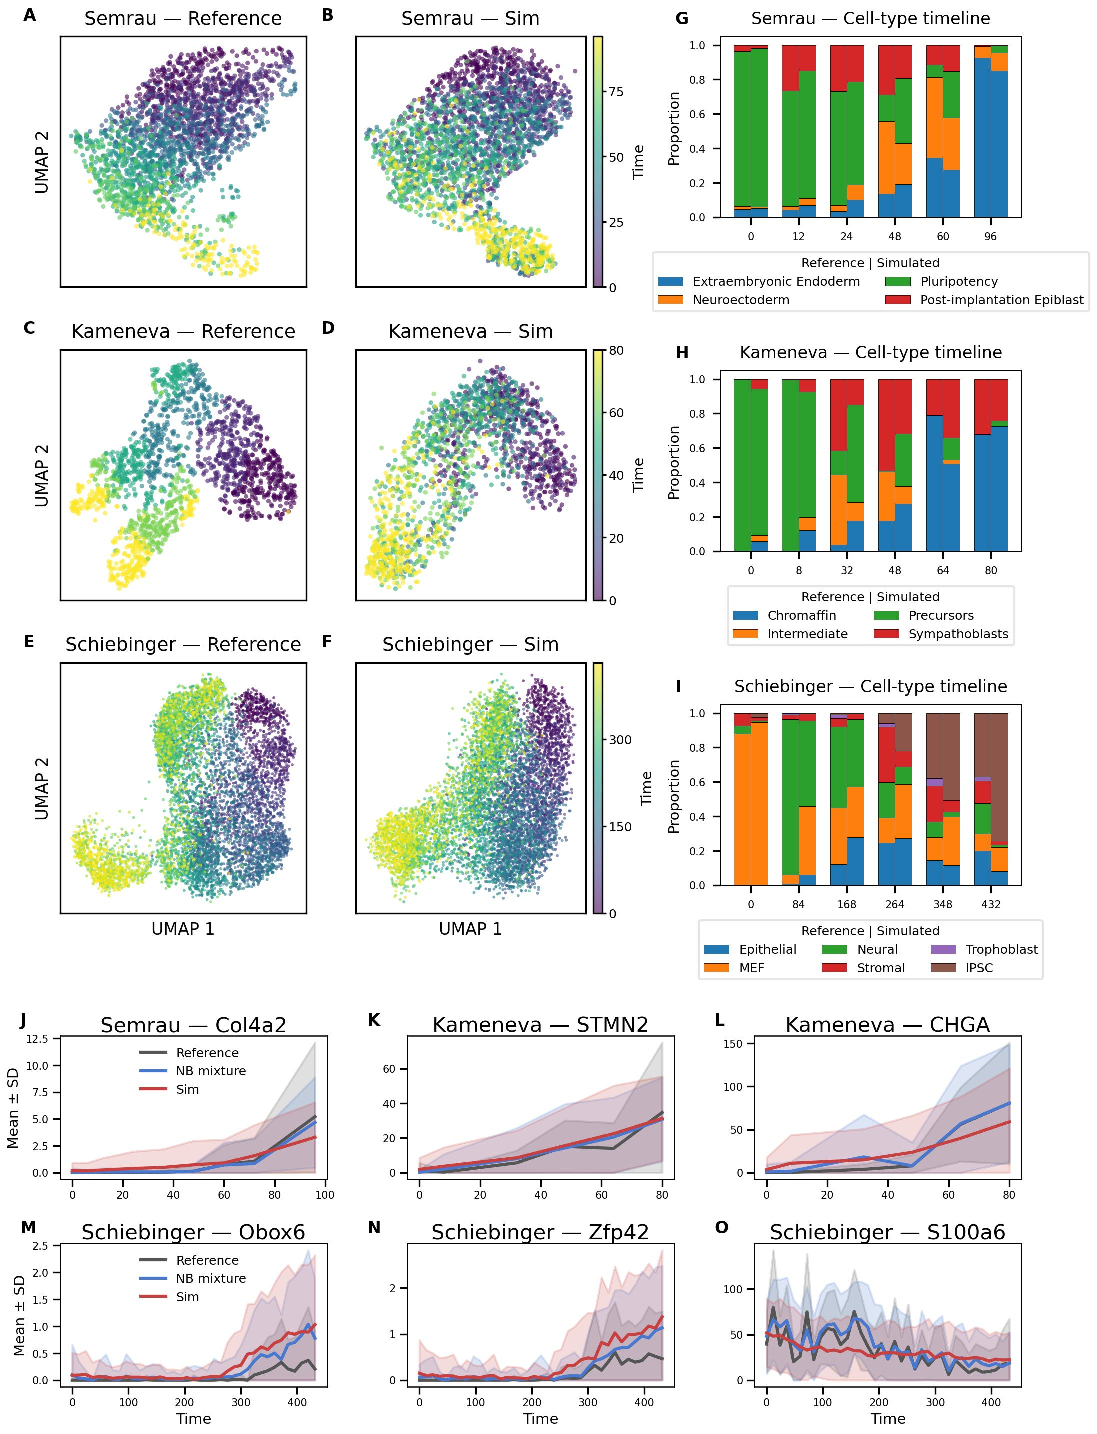
\includegraphics[width=.92\textwidth]{figure_6.pdf}
\caption{CardamomOT performs well as a generative model of protein and mRNA distributions. 
UMAPs of reference (A,C,E) and simulated (B,D,F) data for 3 differentiation datasets. 
Cell type composition for reference and simulated data across timepoints (G--I). Cell type 
composition was inferred for simulated data by a random forest model trained on reference 
data. (J--O) Temporal profiles of mean $\pm$ SD gene expression across all cells for selected key regulators, 
comparing reference data (gray), Negative Binomial reconstruction (blue) and model 
simulations (red), for Col4a2 in the Semrau dataset (J), STMN2 and CHGA in the Kameneva 
dataset (K--L), and Obox6, Zfp42 and S100a6 in the Schiebinger dataset (M--O).}
\label{figure6}
\end{figure}


\begin{figure}
\centering
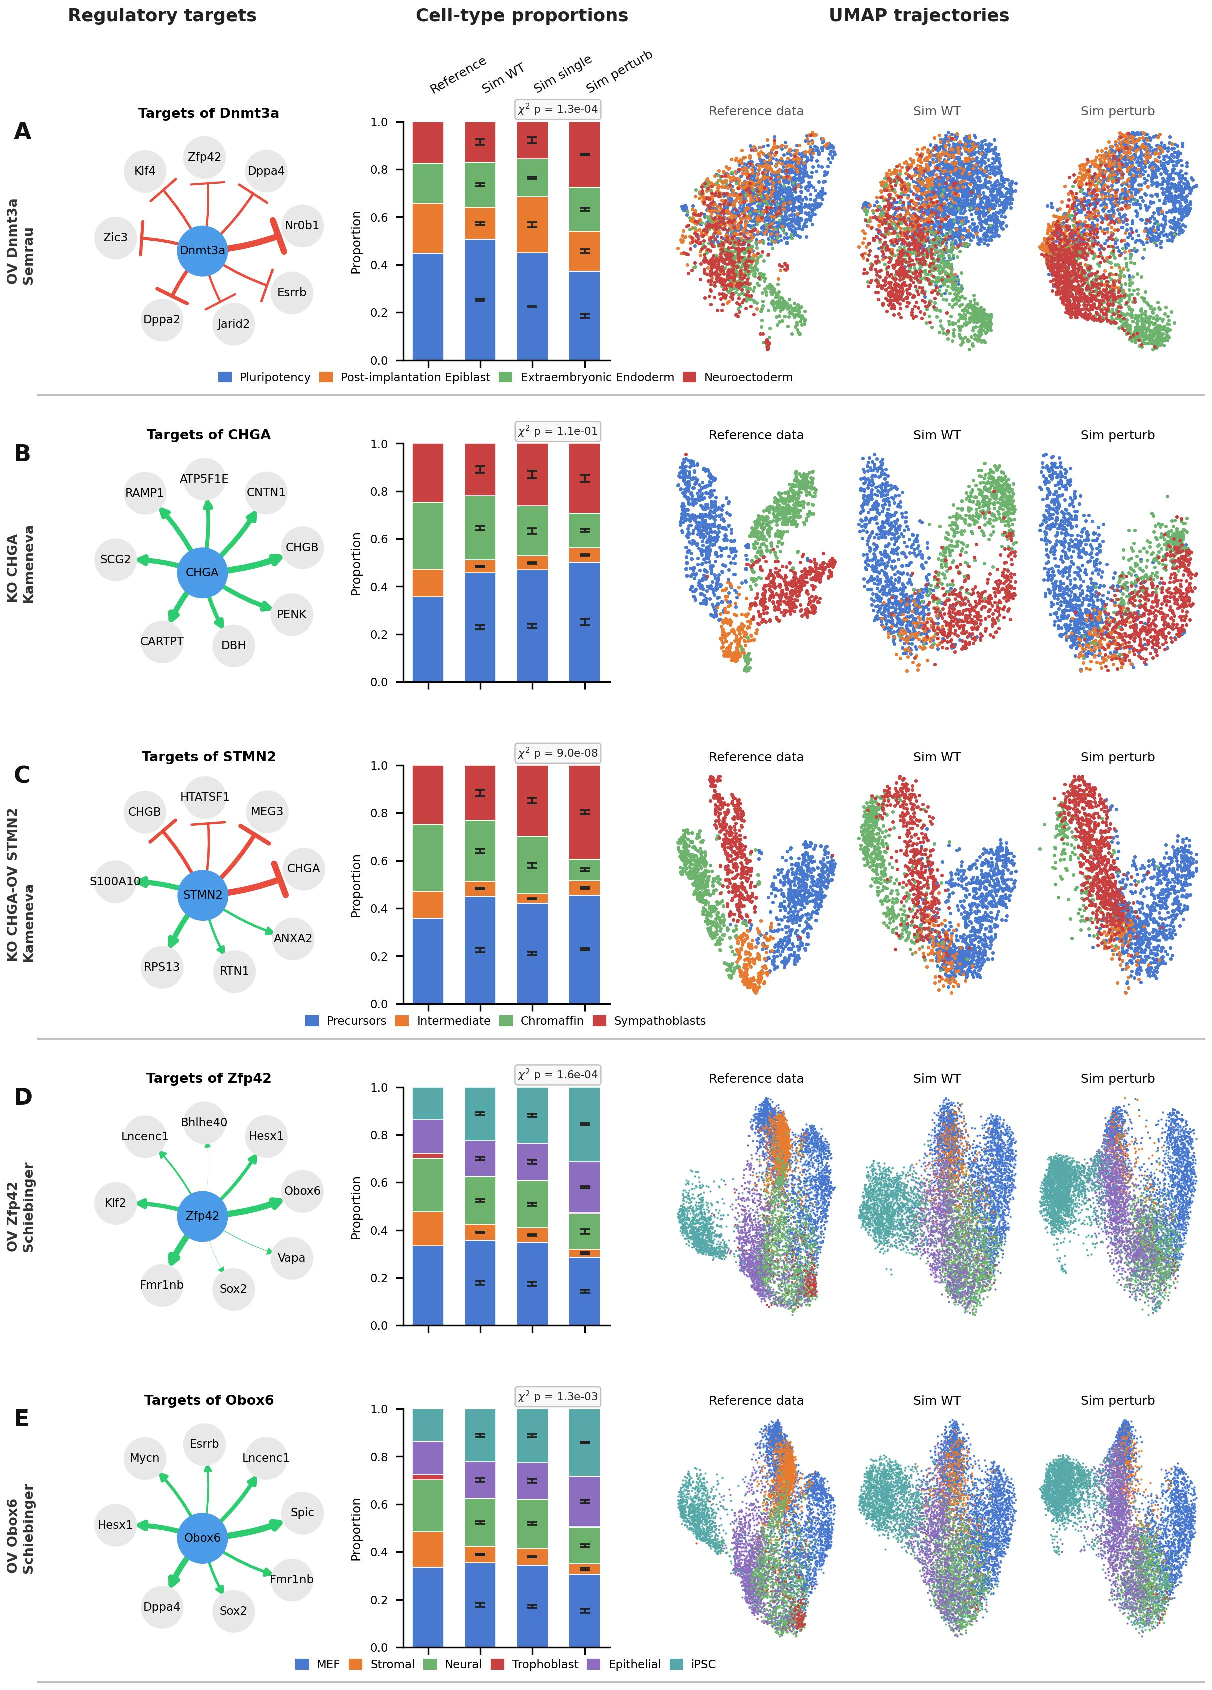
\includegraphics[width=.85\textwidth]{figure_7.pdf}
\caption{In silico perturbations using the inferred GRNs \firstreview{can} recapitulate experimentally 
observed effects. For each perturbation, three 
panels are shown: (left) the regulatory network centered on the perturbed gene, showing 
its top predicted targets with activation (green) and inhibition (red) edges; (middle) 
cell type proportions comparing reference data, wild-type simulation (Sim WT), 
simulation with only the perturbed gene modified (Sim single) and perturbed simulation (Sim perturb); (right) UMAP trajectories 
for reference data, wild-type and perturbed simulations, colored by cell type. The $\chi^2$ test was computed on the base simulated dataset shown here; error bars show the standard deviation of cell-type proportions across $N = 5$ independent stochastic replicates.}
\label{figure7}
\end{figure}

